% ==== Responsável: Rhayanne Borges ====
\chapter{Gerenciamento da Memória Primária}\label{cap:memoria}
O gerenciamento de memória controla a alocação e a desalocação dos endereços da memória. A memória principal é a que a CPU acessa diretamente para executar um programa, e o sistema precisa dividi-la entre os processos protegendo cada um dos demais \cite{tanenbaum2016}.

\section{Tipos de memória e palavras}
A memória principal é formada por DRAM (\textit{Dynamic RAM}). Nela a carga elétrica vaza lentamente, e por isso um circuito de atualização reescreve os dados periodicamente. Já a SRAM (\textit{Static RAM}), usada na memória \textit{cache} da CPU, não precisa ser atualizada, mas é muito mais cara (\autoref{tab:dram-sram}).

\begin{table}[H]
  \centering
  \caption{Comparação entre DRAM e SRAM}\label{tab:dram-sram}
  \begin{tabularx}{\linewidth}{lXX}
    \toprule
    \textbf{Característica} & \textbf{DRAM} & \textbf{SRAM} \\
    \midrule
    Uso típico & Memória principal (1 a 16 GB) & Memória \textit{cache} (1 a 16 MB) \\
    Atualização & Precisa ser reescrita periodicamente & Não precisa \\
    Custo de produção & Menor & Maior \\
    Transferência & Por blocos & Por palavras \\
    \bottomrule
  \end{tabularx}
  \legend{Fonte: adaptado dos slides de \citeonline{bourguet2026processos}.}
\end{table}

As memórias guardam as informações em sequência, em unidades chamadas palavras. Os registradores guardam uma palavra de dados, de 32 ou 64 bits. A largura da palavra limita a memória endereçável: uma CPU de 32 bits usa no máximo $2^{32}$ endereços, ou 4 GB de RAM, e uma de 64 bits usa até $2^{64}$, cerca de 18,4 EB \cite{machado2013}.

\section{Hierarquia e transferências}
A forma de transferência depende do nível de memória 
(\autoref{fig:hierarquia}):

\begin{itemize}
  \item entre a CPU e a \textit{cache} (SRAM), por \textbf{palavras}, de forma rápida;
  
  \item entre a \textit{cache} e a memória principal (DRAM), por \textbf{blocos}, de forma mais lenta;
  
  \item entre a memória principal e a secundária, por \textbf{páginas} ou segmentos, de forma ainda mais lenta.
  
\end{itemize}

\begin{figure}[H]
  \centering
  \caption{Hierarquia de memória e unidades de transferência}\label{fig:hierarquia}
  \begin{tikzpicture}[font=\small, node distance=1.9cm, bx/.style={draw, minimum width=2.2cm, minimum height=1.2cm, align=center}, >=Stealth]
    \node[bx] (cpu) {CPU};
    \node[bx, right=of cpu] (ca) {\textit{Cache}\\(SRAM)};
    \node[bx, right=of ca] (ram) {Memória\\principal\\(DRAM)};
    \node[bx, right=of ram] (hd) {Memória\\secundária};
    \draw[<->] (cpu) -- node[above]{palavra} node[below]{rápida} (ca);
    \draw[<->] (ca) -- node[above]{bloco} node[below]{lenta} (ram);
    \draw[<->] (ram) -- node[above]{página} node[below]{mais lenta} (hd);
  \end{tikzpicture}
  \legend{Fonte: adaptado dos slides de \citeonline{bourguet2026processos}.}
\end{figure}

\section{\textit{Cache} e \textit{buffer}}

Quando o processador quer ler uma palavra, o sistema segue estes passos:
\begin{enumerate}
  \item testa se a palavra está na memória \textit{cache};
  \item se estiver, ela é entregue direto à CPU;
  \item caso contrário, a palavra é buscada na memória principal.
\end{enumerate}
O \textit{caching} acelera o acesso a dados usados repetidamente, e o \textit{buffering} acelera o fluxo de dados da transmissão. A \textit{cache} tem latência menor que 10 ciclos, contra mais de 100 ciclos da RAM\footnote{Disponível em: \url{https://teachcomputerscience.com/memory/}. Acesso em: 19 nov. 2026.}.

\section{Espaço de endereçamento}

Cada processo tem o seu espaço de endereçamento, protegido pelo sistema contra o acesso dos demais. Ele é organizado, do endereço baixo ao alto, em texto (código binário), dados inicializados, BSS (dados não inicializados), \textit{heap} (memória dinâmica) e pilha (\textit{stack}), com variáveis de ambiente no topo. O \textit{heap} cresce para cima e a pilha cresce para baixo, em direção ao espaço livre entre elas.

O comando \texttt{memstat} mostra o uso de memória pelos processos (\autoref{cod:memstat}), e a \autoref{fig:memstat} mostra os valores do exemplo.

\begin{lstlisting}[language=bash, caption={Uso de memória por processo com \texttt{memstat}}, label={cod:memstat}]
$ sudo apt-get install memstat
$ memstat | sort -nr | head -n 20
1082948k: PID 30047 (/usr/lib/firefox/firefox)
1061960k: PID  2795 (/usr/bin/nautilus)
 991736k: PID 29117 (/usr/bin/evince)
\end{lstlisting}

\begin{figure}[H]
  \centering
  \caption{Uso de memória pelos processos do exemplo do \texttt{memstat}}\label{fig:memstat}
  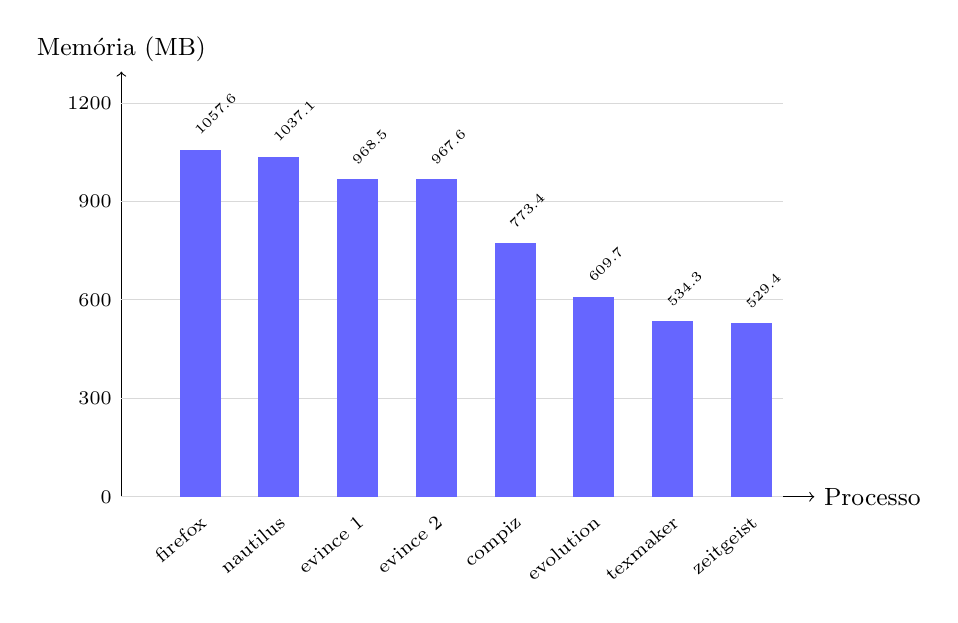
\begin{tikzpicture}[font=\small]
    % Eixos (0 a 1200 MB -> 0 a 5.0 cm)
    \draw[->] (0,0) -- (8.8,0) node[right] {\small Processo};
    \draw[->] (0,0) -- (0,5.4) node[above] {\small Memória (MB)};

    % Linhas de grade e rótulos do eixo Y
    \foreach \val/\y in {0/0, 300/1.25, 600/2.5, 900/3.75, 1200/5.0} {
      \draw[gray!30] (0,\y) -- (8.4,\y);
      \node[left, font=\scriptsize] at (0,\y) {\val};
    }

    % Barras: {posicao_x/altura_cm/valor_mb/nome}
    \foreach \x/\h/\val/\nome in {
      1/4.4067/1057.6/firefox,
      2/4.3213/1037.1/nautilus,
      3/4.0354/968.5/evince 1,
      4/4.0317/967.6/evince 2,
      5/3.2225/773.4/compiz,
      6/2.5404/609.7/evolution,
      7/2.2263/534.3/texmaker,
      8/2.2058/529.4/zeitgeist
    } {
      \fill[blue!60] (\x-0.26,0) rectangle (\x+0.26,\h);
      \node[above, font=\tiny, rotate=45, anchor=south west] at (\x,\h) {\val};
      \node[below, font=\scriptsize, rotate=40, anchor=north east] at (\x,-0.05) {\nome};
    }
  \end{tikzpicture}
  \legend{Fonte: os autores (2026), com valores do \texttt{memstat} dos slides de \citeonline{bourguet2026processos}, convertidos de kB para MB.}
\end{figure}

\section{\textit{Swapping}}

O número de processos ativos pode superar a capacidade da RAM. Para contornar a falta de recursos usa-se a memória virtual: quando a memória enche, processos em espera são transferidos para o disco, na área de \textit{swap}, e trazidos de volta depois (\textit{swap out} e \textit{swap in}). Qualquer dado a processar precisa voltar para a RAM, pois a área de \textit{swap} é apenas um ponto de espera.

A RAM responde em nanossegundos ($10^{-9}$ s) e o disco em milissegundos ($10^{-3}$ s), uma diferença de cerca de um milhão de vezes. Por isso o uso intenso de \textit{swap} é indesejável e, quando frequente, justifica aumentar a RAM \cite{silberschatz2015}.

\section{Paginação}

Paginação e segmentação são técnicas de alocação de memória não contígua. O endereço lógico é gerado pela CPU durante a execução e é virtual, porque não existe fisicamente: ele serve de referência para acessar a memória física. Como o armazenamento não precisa ser sequencial, a paginação elimina a fragmentação externa.

Na paginação o espaço lógico é dividido em páginas de tamanho fixo, e a memória física em quadros do mesmo tamanho. A tradução usa a \textbf{tabela de páginas}, e cada processo tem um PTBR (\textit{Page-Table Base Register}) que aponta para a sua tabela (\autoref{fig:paginacao}). O processo pode ter as páginas de código carregadas sob demanda: ao iniciar, só a parte inicial é carregada, e as demais vêm quando a execução atinge novas regiões.

Em um endereço de 32 bits dividido em 20 + 12 bits, o número da página usa 20 bits ($2^{20} = 1\,048\,576$ páginas) e o deslocamento (\textit{offset}) usa 12 bits ($2^{12} = 4096$ bytes), de modo que cada página tem 4 KB. No exemplo da \autoref{fig:paginacao}, o endereço virtual com página 2 e \textit{offset} 4095 corresponde ao endereço $2 \times 4096 + 4095 = 12287$. A tabela de páginas leva a página 2 ao quadro 15, e o endereço físico fica $15 \times 4096 + 4095 = 65535$.

\begin{figure}[H]
  \centering
  \caption{Tradução de endereço virtual em físico por paginação}\label{fig:paginacao}
  \begin{tikzpicture}[font=\small, >=Stealth, every node/.style={align=center}]
    \node[draw, minimum width=2.4cm, minimum height=0.8cm, fill=red!10] (vp) {página\\2 (20 bits)};
    \node[draw, minimum width=2cm, minimum height=0.8cm, right=0pt of vp, fill=blue!10] (vo) {\textit{offset}\\4095 (12 bits)};
    \node[above=0.1cm of $(vp.north)!0.5!(vo.north)$] {endereço virtual};
    \node[draw, minimum width=3.2cm, minimum height=1.6cm, below=1.6cm of vp] (pt) {tabela de páginas\\(PTBR)\\página 2 $\to$ quadro 15};
    \node[draw, minimum width=2.4cm, minimum height=0.8cm, right=4.2cm of pt, fill=green!10] (fq) {quadro\\15};
    \node[draw, minimum width=2cm, minimum height=0.8cm, right=0pt of fq, fill=blue!10] (fo) {\textit{offset}\\4095};
    \node[above=0.1cm of $(fq.north)!0.5!(fo.north)$] {endereço físico};
    \draw[->] (vp) -- (pt);
    \draw[->] (pt) -- (fq);
    \draw[->] (vo.east) -- ++(0.5,0) |- (fo.north east) ;
  \end{tikzpicture}
  \legend{Fonte: adaptado dos slides de \citeonline{bourguet2026processos}.}
\end{figure}

\section{Segmentação}

Na segmentação o processo é dividido em partições de tamanho variável, os segmentos. Os detalhes de cada um ficam na tabela de segmentação, com a base (endereço inicial na memória física) e o limite (tamanho). O endereço lógico tem número de segmento e \textit{offset}. Se o \textit{offset} é menor que o limite, o endereço físico é a base mais o \textit{offset}; caso contrário ocorre um erro de endereçamento (\textit{trap}). A \autoref{tab:segmentos} traz a tabela do exemplo.

\begin{table}[H]
  \centering
  \caption{Tabela de segmentos do exemplo}\label{tab:segmentos}
  \begin{tabular}{ccc}
    \toprule
    \textbf{Segmento} & \textbf{Base} & \textbf{Limite} \\
    \midrule
    0 & 500 & 600 \\
    1 & 2500 & 800 \\
    2 & 1500 & 400 \\
    3 & 4600 & 200 \\
    4 & 3800 & 400 \\
    \bottomrule
  \end{tabular}
  \legend{Fonte: adaptado dos slides de \citeonline{bourguet2026processos}.}
\end{table}

Por exemplo, o endereço (segmento 2, \textit{offset} 100) vira $1500 + 100 = 1600$. Já o (segmento 2, \textit{offset} 450) gera erro, pois 450 passa do limite 400.

\begin{table}[H]
  \centering
  \caption{Paginação e segmentação}\label{tab:pag-seg}
  \begin{tabularx}{\linewidth}{lXX}
    \toprule
    \textbf{Aspecto} & \textbf{Paginação} & \textbf{Segmentação} \\
    \midrule
    Tamanho das partições & Fixo (páginas) & Variável (segmentos) \\
    Endereço lógico & Página e \textit{offset} & Segmento e \textit{offset} \\
    Tabela & Tabela de páginas (PTBR) & Tabela de segmentos (base e limite) \\
    Fragmentação externa & Eliminada & Pode ocorrer \\
    \bottomrule
  \end{tabularx}
  \legend{Fonte: os autores (2026), com base em \citeonline{bourguet2026processos} e \citeonline{tanenbaum2016}.}
\end{table}

A relação entre a memória primária e o disco é vista na \autoref{cap:memoria-sec}, e os processos que usam essa memória, na \autoref{cap:processos}.